\documentclass{article}
\usepackage[utf8]{inputenc}
\usepackage[top=2cm, bottom=2cm, left=2.5cm, right=2.5cm, footskip=15mm]{geometry}
\usepackage{graphicx}
\usepackage{multicol}
\usepackage{mathptmx}
\usepackage{enumitem}
\usepackage{biblatex}
\usepackage{enumitem}
\usepackage{romannum}

\graphicspath{{images/}}
\setlist[itemize]{itemsep=0pt, parsep=0pt, partopsep=0pt, topsep=0pt}

\let\OLDthebibliography\thebibliography
\renewcommand\thebibliography[1]{
  \OLDthebibliography{#1}
  \setlength{\parskip}{0pt}
  \setlength{\itemsep}{0pt plus 0.3ex}
}

\begin{document}
{\fontfamily{ptm}\selectfont
\begin{multicols}{2}


\pagenumbering{arabic}
\setcounter{page}{57}

\begin{itemize}
\item[] for optimal “stacking” of sc-graphs into processormemory to ensure the subsequent efficiency of
message transmission between processor elements


\item Since the configuration of \textit{logical communication
channels} changes during the processing of sc-constructions, it is also advisable to talk about
the development of algorithms for repositioning
(“defragmentation”) of the sc-construction already
recorded in the processor-memory in order to ensure
the subsequent efficiency of message transmission.
Such reallocation can be performed, for example,
according to a schedule during a period when the
processor-memory is not used for solving other
problems.

\item In addition, if there is a hardware capability, \textit{the physical communication channels} can also be re-switched
in order to approximate their configuration to the
configuration of \textit{logical communication channels}.
\end{itemize}

Let us consider an example of the optimal variant
of writing the simplest \textit{five-element sc-construction} into
the proposed processor-memory within the fine-grained
architecture of \textit{associative semantic computers}.

In Figure 2, the record of some \textit{five-element sc-construction} in the SCg-code is shown.

\begin{center}
    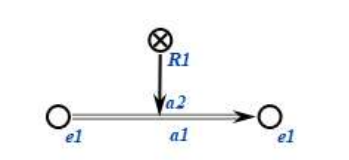
\includegraphics[scale=0.5]{images/aboa.png}
    
    \vspace{+6pt}
    {\small Figure 2. SCg-text. Example of a \textit{five-element sc-construction}}
\end{center}


In Figure 3, an incidence graph for the same \textit{five-element sc-construction} is shown, which allows reducing
the sc-construction to a classical graph with two types
of connections. For clarity, the syntactic types of the
corresponding sc-elements are not shown in the Figure.

\begin{center}
    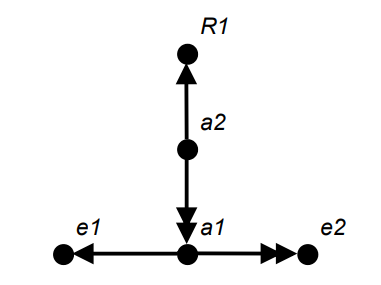
\includegraphics[scale=0.5]{images/aboba.png}
    
    \vspace{+6pt}
    {\small Figure 3. Incidence graph for a \textit{five-element sc-construction}}
\end{center}


In Figure 4, one of the possible optimal options for
recording the resulting incidence graph into   processormemory is shown. Dotted lines show \textit{physical communication channels} between processor elements, solid lines  
show \textit{physical communication channels} corresponding to
\textit{logical communication channels}.  Note that it is advisable
to record element R1 in the \textit{processor element} adjacent  to the \textit{processor element} storing  element e1 or element e2, as shown in the Figure. Due to this, the processor
elements storing the specified sc-elements are directly
connected by a \textit{physical communication channel}, which
simplifies communication in the case of sending messages
via \textit{physical communication channels} without taking into
account \textit{logical communication channels}.

\begin{center}
    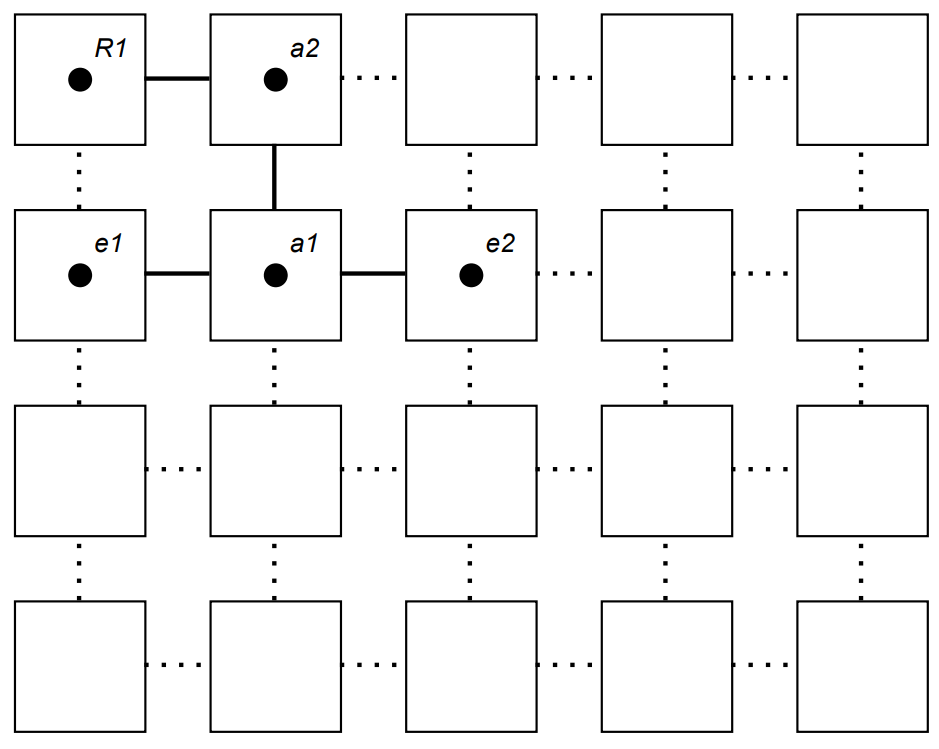
\includegraphics[scale=0.32]{images/abobus.png}
\end{center}
\vspace{+5pt}
{\small Figure 4. Example of stacking an sc-construction into a processormemory}


\begin{center}
    \vspace{+6pt}
    {\large \Romannum{6}. Conclusion}
\end{center}

\vspace{-2pt}
In the article, the disadvantages of the currently
dominant von Neumann architecture of computer systems
as a basis for building-up intelligent computer systems of
a new generation are considered, the analysis of modern
approaches to the development of hardware architectures
that eliminate some of these disadvantages is carried
out, the need for the development of fundamentally
new hardware architectures representing a hardware
implementation of ostis-platforms – \textit{associative semantic
computers} – is demonstrated.

The general principles underlying \textit{associative semantic
computers} are proposed, three possible variants of the
architecture of such computers are considered, their
advantages and disadvantages are represented.

Further development of the approaches proposed in
the work requires solving a number of problems, both
technical and organizational ones:
\vspace{+3pt}
\begin{itemize}
    \item development of a wave language for recording microprograms, that are exchanged between processor
    elements and run by these processor elements;
    
    \item development of a language for writing programs
for controlling the exchange of micro-programs and
managing the queue of micro-programs;

    \item organization of active participation of specialists
in the field of microelectronics in clarifying the
principles of implementation of processor elements
and processor-memory in general, clarifying the
element base and lower-level architectural features
of \textit{associative semantic computers};
    \item development of algorithms for optimizing the ways
of recording sc-constructions to processor-memory
and repositioning already recorded sc-constructions
in order to ensure the subsequent efficiency of
message transmission between processor elements;
    \item clarification of the typology of information processes
in the processor-memory, their features, and the
corresponding typology of labels;
    \item clarification of the principles of implementing multiagent knowledge processing within the processormemory, in particular, the development of principles
for implementing event-based information processing
in such memory.
\end{itemize}

\begin{center}
    {\fontfamily{cmtt}\selectfont {\large A}CKNOWLEDGEMENT}
\end{center}


The author would like to thank the research groups of
the Departments of Intelligent Information Technologies
of the Belarusian State University of Informatics and
Radioelectronics and the Brest State Technical University
for their help in the work and valuable comments.

\begin{center}
    {\fontfamily{cmtt}\selectfont {\large R}EFERENCES}
    \vspace{-30pt}
\end{center}

{\footnotesize
\renewcommand\refname{}
\begin{thebibliography}{65}
    \item J. von Neumann, “First draft of a report on the EDVAC,” \textit{IEEE
Annals of the History of Computing}, vol. 15, no. 4, pp. 27–75,
1993.
    \item M. D. Godfrey and D. F. Hendry, “The computer as
von Neumann planned it,” \textit{IEEE Annals of the History of
Computing}, vol. 15, no. 1, pp. 11–21, 1993. [Online]. Available:
https://doi.org/10.1109/85.194088

    \item V. Glushkov [et al.], \textit{Rekursivnye mashiny i vychislitel’naya
tekhnika [Recursive machines and computer engineering]}. IC of
the Academy of Sciences of the Ukrainian SSR, 1974.
    \item J. Aylif, \textit{Principy postroeniya bazovoj mashiny [Principles of
building the basic machine]}. Mir, 1973.
    \item  D. Moldovan, W. Lee, C. Lin, and M. Chung, “SNAP: Parallel
Processing Applied to AI,” \textit{Computer}, pp. 39–49, 1992.
    \item Y. Chu, “Evolution of computer memory structure,” \textit{Proc. National
Computer Conf}. AFIPS Press, pp. 733–748, 1976.
    \item L. Kalinichenko and V. Ryvkin, \textit{Mashiny baz dannyh i znanij
[Database and knowledge machines]}. M. : Nauka, 1990, (In
Russ.).
    \item J. Martin, \textit{Organizaciya baz dannyh v vychislitel’nyh sistemah:
Per. s angl. [Organization of databases in computing systems:
Trans. from English]}. Mir, 1980.
    \item E. Ozkarahan, \textit{Mashiny baz dannyh i upravlenie bazami dannyh
[Database machines and database control]}. Mir, 1989.
    \item T. Kohonen, \textit{Associativnaya pamyat’: Per. s angl. [Associative
memory: Trans. from English]}. Mir, 1980, (In Russ.).
    \item V. Ignatushchenko, “K postanovke zadachi povysheniya effektivnosti vychislitel’nyh sistem na osnove associativnyh metodov
obrabotki informacii [To the formulation of the problem of
increasing the efficiency of computing systems based on associative methods of information processing],” \textit{Voprosy kibernetiki.
Mnogoprocessornye vychislitel’nye sistemy s perestraivaemoj
strukturoj (Arhitektura. Struktura. Primeneniya) [Questions of
cybernetics. Multiprocessor computing systems with a tunable
structure (Architecture. Structure. Applications)]}, pp. 14–21, 1981.
    \item S. Berkovich, Yu. Kochin, and V. Molchanov, “Ob effektivnosti
primeneniya associativnoj pamyati v vychislitel’nyh procedurah
[On the effectiveness of using associative memory in computational
procedures],” \textit{Vychislitel’nye sistemy. Vyp. 62. [Computing systems.
Issue 62.]}, pp. 97–105, 1975.
    \item M. Aizerman, L. Gusev, S. Petrov, and I. Smirnova, “Dinamicheskij podhod k analizu struktur, opisyvaemyh grafami (osnovy
grafodinamiki) [Dynamic approach to the analysis of structures
described by graphs (fundamentals of graph dynamics)],” \textit{Avtomatika i telemekhanika [Automation and telemechanics]}, no.
7/8, pp. 135–151/123–136, 1977.
    \item  G. Marchuk [et al.], \textit{Modul’naya asinhronnaya
razvivayushchayasya sistema: V 2-h ch. [Modular asynchronous
developing system: In 2 parts]}. Academy of Sciences of the
USSR. Sib.department. Computing Center, 1978.
    \item
    I. Prangishvili and G. Stetsyura, “Sovremennoe sostoyanie problemy sozdaniya EVM s netradicionnoj strukturoj i arhitekturoj,
upravlyaemyh potokom dannyh [Current state of the problem
of creating computers with an unconventional structure and
architecture controlled by the data flow],” \textit{Izmerenie, kontrol’,
avtomatizaciya [Measurement, control, automation]}, no. 1, pp.
36–48, 1981.
    \item Y. Zatuliver and I. Medvedev, “Voprosy postroeniya i mnogoprocessornoj realizacii yazyka strukturno-parallel’nogo programmirovaniya s upravleniem potokami dannyh [Issues of
building and multiprocessor implementation of a structurally
parallel programming language with data flow control],” \textit{Voprosy kibernetiki. Mnogoprocessornye vychislitel’nye sistemy s
perestraivaemoj strukturoj (Arhitektura. Struktura. Primeneniya)
[Issues of cybernetics. Multiprocessor computing systems with
a tunable structure (Architecture. Structure. Applications)]}, pp.
123–166, 1981.
    \item
    W.B. Ackerman, “Data flow language,” \textit{Proc. National Computer
Conf. AFIPS Press}, pp. 1087–1095, 1979.
    \item G. Myers, \textit{Arhitektura sovremennyh EVM: V 2-h kn. Kn. 2. / Per.
s angl. [Architecture of modern computers: In 2 books. Book 2. /
Transl. from English.]}. Mir, 1985.
    \item V. Glushkov, “Fundamental’nye issledovaniya i tekhnologiya
programmirovaniya [Fundamental research and programming
technology],” \textit{Programmirovanie [Programming]}, no. 2, pp. 3–13,
1980.
    \item V. Glushkov, S. Pogrebinsky, and Z. Rabinovich, “O razvitii struktur mul’tiprocessornyh EVM s interpretaciej yazykov
vysokogo urovnya [On the development of multiprocessor computer structures with interpretation of high-level languages],”
\textit{Upravlyayushchie mashiny i sistemy [Control machines and
systems]}, no. 6, pp. 61–66, 1978.
    \item Z. Rabinovich, “O koncepcii mashinnogo intellekta [About the
concept of machine intelligence],” \textit{Kibernetika i sistemnyj analiz
[Cybernetics and system analysis]}, no. 2, pp. 163–173, 1995.
    \item I. Zadykhailo [et al.], \textit{Proekt associativnogo parallel’nogo processora na CMD, orientirovannogo na podderzhku relyacionnyh baz
dannyh [Project of an associative parallel processor on the CMD,
focused on the support of relational databases]}. Academy of
Sciences of the USSR. Institute of applied mathematics, 1979.

    \item S. Schuster, H. Nguyen, E. Oskarachan, K. Smith, “RAP.2 – an
associative processor for databases and its applications,” \textsl{IEEE}
\textit{Trans. on Computers}, no. 6, pp. 446–458, 1979.

    \item E. Suvorov and Ya. Fet, “Processory baz dannyh [Database processors],” \textit{Iss. of the USSR Academy of Sciences. Tech. Cybernet}.,
no. 6, pp. 63–75, 1985.
    \item  H.J. Brukle, “High level language oriented hardware and post –
von Neumann era,” \textit{Proc. 5-th Symp Computer Architecture}, pp.
60–65, 1978.
    \item Y. Chu, “Architecture of a hardware data interpreter,” \textit{Proc. 4-th
IEEE Symp. on Computer Architecture}, pp. 1–9, 1977.
    \item T. Kohonen, \textit{Associativnye zapominayushchie ustrojstva: Per. s
angl. [Associative storage devices: Trans. from English.]}. Mir,
1982.
    \item K. Foster, \textit{Associativnye parallel’nye processory [Associative
parallel processors]}. Energoizdat, 1981.
    \item A. Ershov, \textit{Algoritmy, matematicheskoe obespechenie i arhitektura
mnogoprocessornyh vychislitel’nyh sistem [Algorithms, mathematical support, and architecture of multiprocessor computing
systems]}. Nauka, 1982.
    \item L. Berstein, V. Lisyak, and V.Rabinovich, “Odnorodnaya programmiruemaya struktura dlya resheniya kombinatorno-logicheskih
zadach na grafah i gipergrafah [Homogeneous programmable
structure for solving combinatorial logic problems on graphs and
hypergraphs],” \textit{Metody rascheta i avtomatizaciya proektirovaniya
ustrojstv v mikroelektronnyh CVM [Calculation methods and
automation of device design in microelectronic digital computers]},
pp. 39–52, 1975.
    \item V. Vasiliev and E. Raldugin, \textit{Elektronnye modeli zadach na
grafah [Electronic models of graph problems]}. Naukova dumka
[Scientific thought], 1987.
    \item P. Sapaty, “Aktivnoe informacionnoe pole kak model’ strukturnogo
resheniya zadach na grafah i setyah [Active information field as
a model of structural problem solving on graphs and networks],”
\textit{Iss. of the USSR Academy of Sciences. Tech. Cybernet}., no. 5, pp.
184–208, 1984.
    \item A. Popov, “Primenenie geterogennoj vychislitel’noj sistemy s
naborom komand diskretnoj matematiki dlya resheniya zadach
na grafah [Application of a heterogeneous computing system
with a set of discrete mathematics commands for solving
graph problems],” \textit{Informacionnye tekhnologii [Information
technologies]}, vol. 25, no. 11, pp. 682–690, 2019, (In Russ.).
    \item A. Popov, “Principy organizacii geterogennoj vychislitel’noj
sistemy s naborom komand diskretnoj matematiki [Principles
of organization of a heterogeneous computing system with a set
of discrete mathematics commands],” \textit{Informacionnye tekhnologii
[Information technologies]}, vol. 26, no. 2, pp. 67–79, 2020, (In
Russ.).
    \item J. Zhang, S. Khoram, and J. J. Li, “Boosting the Performance of
FPGA-based Graph Processor using Hybrid Memory Cube: A Case
for Breadth First Search,” \textit{Proceedings of the 2017 ACM/SIGDA
International Symposium on Field-Programmable Gate Arrays},
2017.
    \item Y. Hu, Y. Du, E. Ustun, and Z. Zhang, “GraphLily: Accelerating Graph Linear Algebra on HBM-Equipped FPGAs,” \textit{2021
IEEE/ACM International Conference On Computer Aided Design
(ICCAD)}, pp. 1–9, 2021.
    \item W. S. Song, V. Gleyzer, A. Lomakin, and J. Kepner,
“Novel graph processor architecture, prototype system, and
results,” in \textit{2016 IEEE High Performance Extreme Computing
Conference (HPEC)}. IEEE, Sep. 2016. [Online]. Available:
https://doi.org/10.1109/hpec.2016.7761635
    \item I. V. Afanasyev, V. V. Voevodin, K. Komatsu, and H. Kobayashi,
“VGL: a high-performance graph processing framework for the
NEC SX-aurora TSUBASA vector architecture,” \textit{The Journal
of Supercomputing}, vol. 77, no. 8, pp. 8694–8715, Jan. 2021.
[Online]. Available: https://doi.org/10.1007/s11227-020-03564-9
    \item M. Weinzweig, \textit{Obuchayushchayasya sistema iskusstvennogo
intellekta s associativnoj pamyat’yu-processorom [Learning Artificial Intelligence system with associative memory processor]}.
USSR Academy of Sciences, Scientific Council. according to the
complex. probl. “Cybernetics”, 1980.
    \item M. Weinzweig and M. Polyakova, “Mekhanizm myshleniya i
modelirovanie ego raboty v real’nom vremeni [Mechanism of
thinking and modeling its work in real time],” \textit{Intellektual’nye
processy i ih modelirovanie [Intelligent processes and their
modeling]}, pp. 208 – 229, 1987.

    \item S. Somsubhra, “Reconfigurable semantic processor,” Oct 2006.
    
    \item Z. Rabinovich, “Nekotoryj bionicheskij podhod k strukturnomu
modelirovaniyu celenapravlennogo myshleniya [Some bionic approach to structural modeling of purposeful thinking],” \textit{Kibernetika
[Cybernetics]}, no. 2, pp. 115–118, 1979.

    \item ——, “Razvitie struktur universal’nyh EVM v svyazi s problemami
avtomatizacii nauchnyh issledovanij [Development of universal
computer structures in connection with the problems of automation
of scientific research],” \textit{Avtomatika [Automation]}, no. 5, pp. 63–72,
1979.
    \item V. Gladun, \textit{Evristicheskij poisk v slozhnyh sredah [Heuristic search
in complex environments]}. Naukova dumka [Scientific thought],
1977.
    \item ——, \textit{Planirovanie reshenij [Planning solutions]}. Naukova dumka
[Scientific thought], 1987.
    \item N. Amosov, A. Kasatkin, L. Kasatkina, and S. Talaev, \textit{Avtomaty
i razumnoe povedenie [Automata and reasonable behavior]}.
Naukova dumka [Scientific thought], 1973.

    \item E. Zolotov and I. Kuznetsov, \textit{Rasshiryayushchiesya sistemy
aktivnogo dialoga [Expanding active dialogue systems]}. Nauka,
1982.
    \item A. Galushkin, “Sovremennye napravleniya razvitiya
nejrokomp’yuternyh tekhnologij v Rossii [Modern directions of
development of neurocomputer technologies in Russia],” \textit{Otkrytye
sistemy [Open systems]}, no. 4, pp. 25–28, 1997, (In Russ.).
    \item R. Hecht-Nielsen, “Nejrokomp’yuting: istoriya, sostoyanie, perspektivy [Neurocomputing: history, state, prospects],” \textit{Otkrytye
sistemy [Open systems]}, no. 4, pp. 23–28, 1998.

    \item L. Komartsova and A. Maksimov, \textit{Nejrokomp’yutery. - 2-e izd.
[Neurocomputers. – 2nd ed.]}, ser. Informatika v tekhnicheskom
universitete [Computer Science at the Technical University].
Moscow: Bauman Moscow State Technical University, 2004.
    \item (2022, Dec) USB Accelerator | Coral. [Online]. Available:
https://coral.ai/products/accelerator/
    \item M. Moussa, A. Savich, and S. Areibi, “Architecture, system and
method for artificial neural network implementation,” Jun 2013.
    \item “Nejromorfnyj processor “Altaj” Neuromorphic processor “Altai”,”
mode of access: https://motivnt.ru/neurochip-altai/. — Date of
access: 29.03.2023.
    \item J. D. Allen, J. Philip, and L. Butler, “Parallel machine architecture
for production rule systems,” Jun 1989.
    \item “CUDA Toolkit,” mode of access: https://developer.nvidia.com/
cuda-toolkit. — Date of access: 29.03.2023.

    \item “OpenCL,” mode of access: https://www.khronos.org/opencl/. —
Date of access: 29.03.2023.
    \item H.-N. Tran and E. Cambria, “A survey of graph processing
on graphics processing units,” \textit{The Journal of Supercomputing},
vol. 74, no. 5, pp. 2086–2115, Jan. 2018. [Online]. Available:
https://doi.org/10.1007/s11227-017-2225-1

    \item X. Shi, Z. Zheng, Y. Zhou, H. Jin, L. He, B. Liu, and
Q.-S. Hua, “Graph processing on GPUs,” \textit{ACM Computing
Surveys}, vol. 50, no. 6, pp. 1–35, Nov. 2018. [Online]. Available:
https://doi.org/10.1145/3128571

    \item Y. Lü, H. Guo, L. Huang, Q. Yu, L. Shen, N. Xiao, and
Z. Wang, “GraphPEG,” \textit{ACM Transactions on Architecture and
Code Optimization}, vol. 18, no. 3, pp. 1–24, Sep. 2021. [Online].
Available: https://doi.org/10.1145/3450440
    \item V. Golenkov, “Strukturnaya organizaciya i pererabotka informacii
v elektronnyh matematicheskih mashinah, upravlyaemyh potokom
slozhnostrukturirovannyh dannyh [Structural organization and
processing of information in electronic mathematical machines
controlled by the flow of complex structured data],” PhD diss.:
05.13.01 ; 05.13.13, Minsk, 1996.
    \item ——, \textit{Parallel’nyj grafovyj komp’yuter (PGC), orientirovannyj
na reshenie zadach iskusstvennogo intellekta, i ego primenenie
(Preprint; No 2) [Parallel graph computer (PGC), focused
on solving artificial intelligence problems, and its application
(Preprint; No. 2)]}. Institute of Technical Cybernetics, 1994.

    \item V. Golenkov [et al.], \textit{Terminal’nyj modul’ parallel’nogo grafovogo
komp’yutera (PGC): Interfejs s pol’zovatelem i processornymi
modulyami, struktura, logicheskaya organizaciya: materialy po
matematicheskomu obespecheniyu EVM [Terminal module of a
parallel graph computer (PGC): User interface and processor
modules, structure, logical organization: materials on computer
mathematical support]}. Institute of Technical Cybernetics, 1994.
    \item V. Golenkov, “Grafodinamicheskie modeli i metody parallel’noj
asinhronnoj pererabotki informacii v intellektual’nyh sistemah
[Graphodynamic models and methods of parallel asynchronous
processing of information in intelligent systems],” Doct. diss.:
05.13.11 ; 05.13.17, Minsk, 1996, 396 p.
    \item P. Gaponov, “Modeli i metody parallel’noj asinhronnoj pererabotki
informacii v grafodinamicheskoj associativnoj pamyati [Models
and methods of parallel asynchronous processing of information in
graphodynamic associative memory],” PhD diss.: 05.13.11, Minsk,
2000, 114 p.

    \item V. Kuzmitsky, “Principy postroeniya grafodinamicheskogo
parallel’nogo komp’yutera, orientirovannogo na reshenie zadach
iskusstvennogo intellekta [Principles of building a graphodynamic
parallel computer focused on solving artificial intelligence
problems],” PhD diss.: 05.13.11, Minsk, 2000, 236 p.


\end{thebibliography}
}

\end{multicols}
}
\end{document}
